\section{Why Does Adaptive Selection Not Help?}\label{sec:analysis}

\para{What the selector chose}
Over the 420 \ars{} folds, the minority classes produced 970 clusters. The resampler applied was SMOTE-Tomek for 33\%
of them, SMOTE for 30\%, SMOTE-ENN for 29\%, ADASYN for 6\% and random oversampling for 2\%.
Figure~\ref{fig:usage} shows that the choice is effectively made per \emph{dataset}. On 11 datasets, one resampler is
used for every cluster in every fold. The clustering does split the minority class, into 1.8 clusters on average and
into several clusters in 57\% of folds, but clusters of the same dataset receive similar scores and hence the same
rule. DBSCAN always returned a single cluster, yet ARS with DBSCAN matches the $k$-means version (F1 rank 4.20 versus
4.79). Per-cluster heterogeneity is not what drives performance.

\begin{figure}
  \centering
  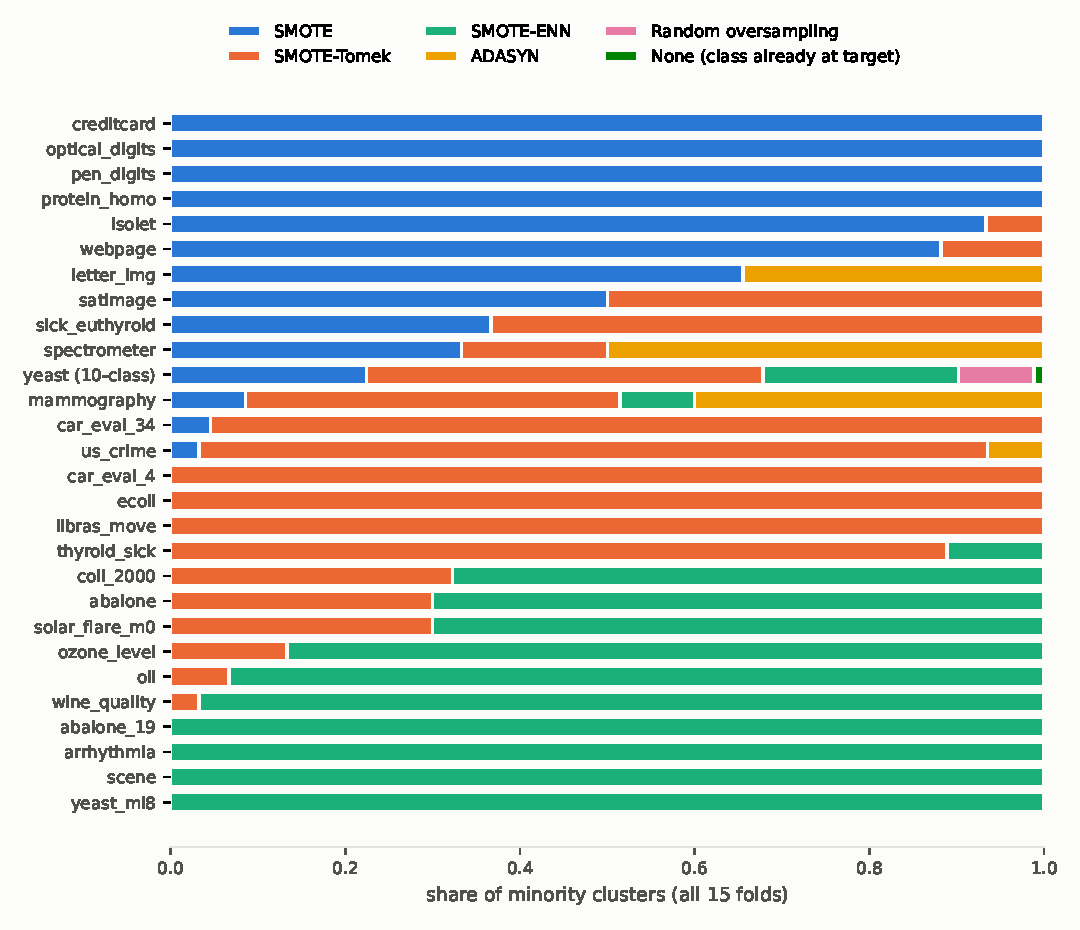
\includegraphics[width=\usagefigwidth]{figures/resampler_usage.pdf}
  \caption{Resampler applied by \ars{} per minority cluster, as a share over the 15 folds of each dataset. Most
  datasets are dominated by one resampler.}
  \label{fig:usage}
\end{figure}

\para{SMOTE-Tomek is SMOTE}
After 1:1 SMOTE, synthetic points fill the minority region so densely that almost no cross-class nearest-neighbour
pairs (Tomek links) remain. Global SMOTE-Tomek gave \emph{bit-identical} results to SMOTE on 280 of 420 folds, and on
all folds of 12 datasets, while its cleaning step cost up to 114\,s per creditcard fold. \ars{}'s most frequent choice
is therefore effectively SMOTE, and its real candidate pool is dominated by SMOTE.

\para{Confidence weighting is equal weighting}
The three learners reach similar validation AUC-PR, so the weights of Eq.~\ref{eq:weights} stay near $1/3$. The
median gap between the largest and smallest weight is 0.022 (90th percentile 0.10). \ars{} and equal-weight averaging
give identical metrics on 159 of 420 folds (mean AUC-PR difference $+0.0001$). The weights have nothing to correct
when the learners are this strong and this similar. Meta-learner stacking is also equivalent, at 4.6$\times$ the
compute (5.7 versus 1.2 hours).

\paragraph{When does resampling help at all?}
Figure~\ref{fig:benefit} plots, per dataset, the gain from resampling over the same ensemble without resampling,
against the minority-class size:
\begin{itemize}
  \item \textbf{$\leq75$ minority samples (10 datasets):} SMOTE improves AUC-PR on 8 (mean $+0.012$); \ars{} on 8
        (mean $+0.005$).
  \item \textbf{$>75$ minority samples (18 datasets):} SMOTE improves AUC-PR on only 5 (mean $-0.009$); \ars{} on 4
        (mean $-0.012$).
\end{itemize}
F1 and MCC show the same pattern. The Spearman correlations between gain and minority size are negative throughout
(e.g.\ $\rho=-0.48$, $p=0.010$ for \ars{} on F1), but none survives Holm correction over the 24 tests we ran. The
imbalance ratio itself is not predictive. The absolute number of minority examples, not their proportion, appears to
limit a strong learner. We report this as a consistent trend, not a confirmed effect.

\begin{widefigure}
  \centering
  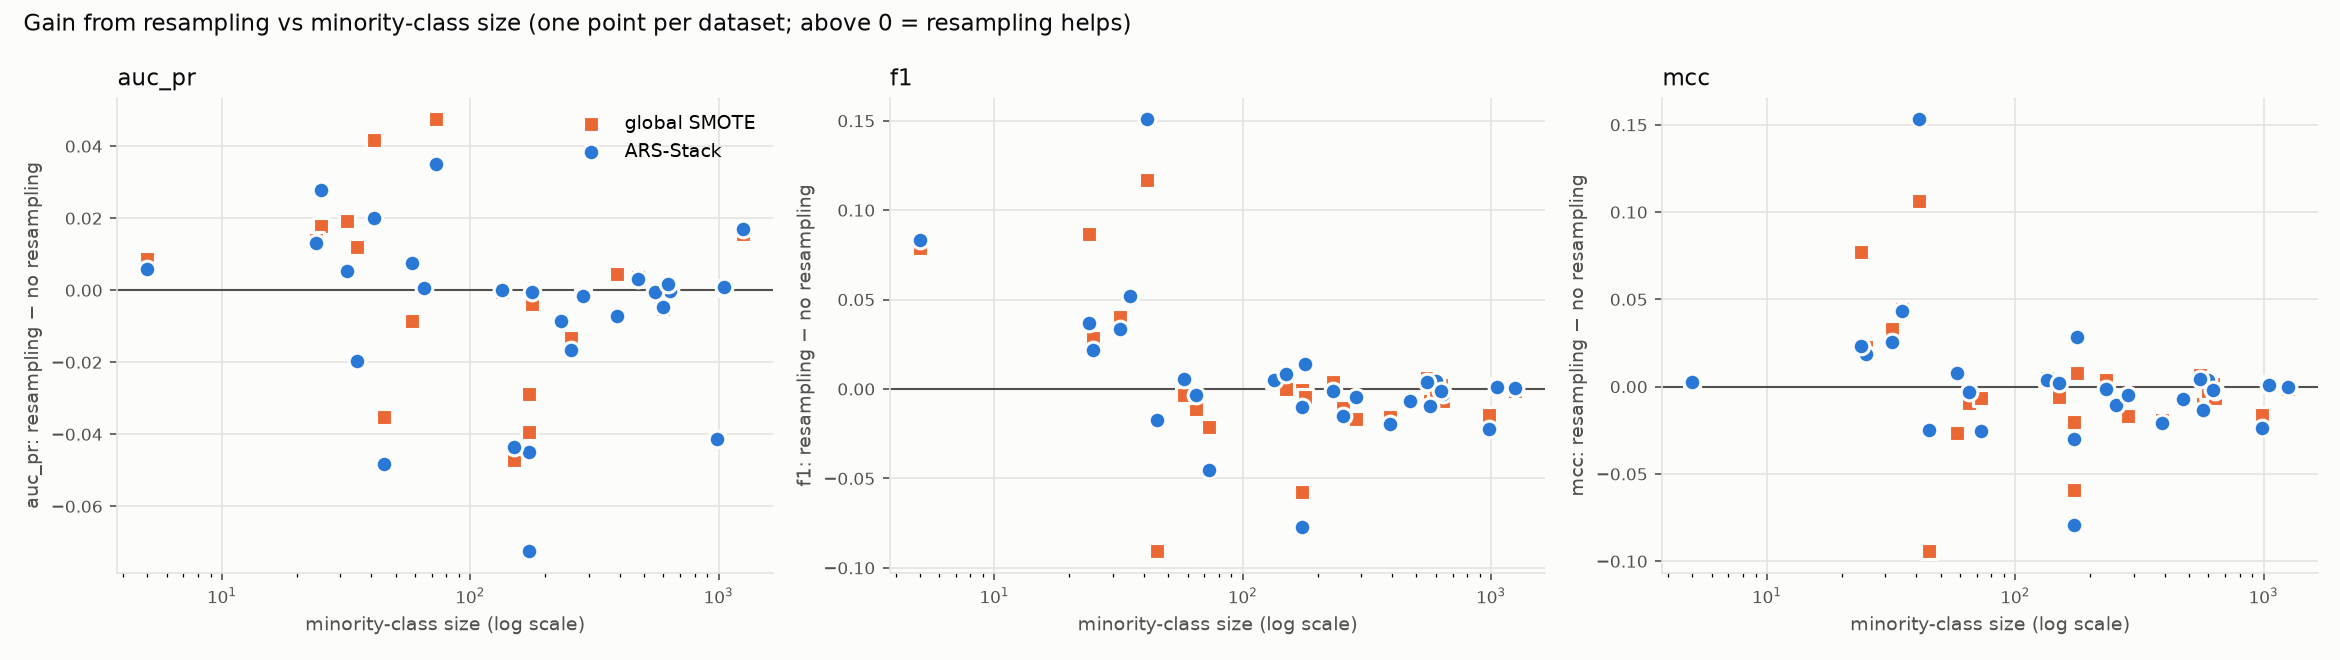
\includegraphics[width=\linewidth]{figures/resampling_benefit.png}
  \caption{Gain from resampling (global SMOTE, \ars{}) over no resampling versus minority-class size (log scale), one
  point per dataset. Resampling tends to help below about 75 minority samples and to be neutral or harmful above.}
  \label{fig:benefit}
\end{widefigure}

\para{Pilot: validated selection}
Perhaps hand-written rules are just a poor selector. To test this, we replaced them with \emph{validated selection}:
the method (no resampling, global SMOTE, or \ars{}'s adaptive resampling) and the amount
($\beta\in\{0.1,0.25,0.5,1\}$) are chosen jointly by 3-fold inner cross-validation on the training data (LightGBM
AUC-PR), and a single cluster is kept unless the silhouette score exceeds 0.25. A control, SMOTE-Select, runs the same
search without the adaptive option.

To avoid tuning on the reported benchmark, the datasets were split into 14 development and 14 held-out sets,
stratified by minority size and imbalance. The pilot used 12 development datasets and 5 folds, all on one machine.
That matters: repeating an identical configuration on different hardware moved AUC-PR by 0.007 on average, as much as
the effects studied.

Table~\ref{tab:pilot} shows that validated selection repairs \ars{}'s deficit ($+0.0095$ AUC-PR over the rule-based
version) but only reaches the baselines: $+0.0006$ over No resampling (5 wins, 7 losses) and identical to SMOTE-Select.
The adaptive option adds nothing, and the chosen configurations were spread over all candidates, a sign that they
perform alike. The headroom is small in any case: an oracle picking the best of No resampling, SMOTE, SMOTE-Tomek and
\ars{} per dataset in hindsight gains only $+0.008$ mean AUC-PR over No resampling. We therefore did not spend a
second full run on this design.

\begin{table}
  \centering
  \caption{Validated-selection pilot on 12 development datasets (5 folds, one machine): mean score (average rank among
  the five variants).}
  \label{tab:pilot}
  \scriptsize
  \setlength{\tabcolsep}{2pt}
  \resizebox{\linewidth}{!}{\begin{tabular}{lrrrr}
\toprule
Variant & F1 & AUC-PR & G-mean & MCC \\
\midrule
No resampling & 0.4919 (2.92) & 0.5301 (2.67) & 0.6944 (2.92) & 0.4696 (2.92) \\
SMOTE & 0.4854 (3.67) & 0.5290 (3.08) & 0.6810 (3.75) & 0.4602 (3.75) \\
ARS-Stack & 0.4920 (2.92) & 0.5212 (3.50) & 0.6937 (3.08) & 0.4651 (3.08) \\
SMOTE-Select (validated) & 0.4951 (2.71) & 0.5307 (2.83) & 0.6989 (2.46) & 0.4705 (2.62) \\
ARS-Select (validated) & 0.4921 (2.79) & 0.5307 (2.92) & 0.6907 (2.79) & 0.4669 (2.62) \\
\bottomrule
\end{tabular}
}
\end{table}
